% !Mode:: "TeX::UTF-8"
\documentclass{svk_en}
%% ak pisete po slovensky, pouzijete namiesto horneho riadku
%% \documentclass{svk_sk}

\usepackage{algorithm}      % For the float environment (optional)
\usepackage{algpseudocode}
\usepackage{amssymb}
\usepackage{amsmath}
\usepackage{bm}

\begin{document}
\title{Segment focused portfolio optimization \\ based on machine learning predictions}

\author{Marek Šugár
\email{sugar11@uniba.sk}}

%% vsimnite si, ze u autorov sa nepisu tituly
%% prikaz \inst sluzi ako odkaz do zoznamu institucii
%% (vid. nizsie)

%% ak je skolitel/ka prace sucastne autorom, oznacte ho/ju uvedenym sposobom
%% ak praca ma skolitela, ktory ale nie je autorom, uvedte to cez nasledujuci prikaz
\supervisor{Samuel Rosa \inst{1}
\email{samuel.rosa@fmph.uniba.sk}}
%% ak praca nema skolitela, jednoducho vynechajte


%% nasleduje kratka verzia nazvu clanku a 
%% zoznam autorov (bez krstnych mien)
%% tieto informacie sa zobrazuju v hlavicke
\titlerunning{On portfolio optimization based on machine learning predictions}
\authorrunning{Šugár}

\institute{
      Department of Applied Mathematics and Statistics,
      FMFI UK,
      Mlynská dolina,
      842~48~Bratislava}

\maketitle

\begin{abstract}
In this paper, we present a complex analysis of approaches to portfolio optimization based on predictions made by machine learning (ML)
algorithms. We compare the prediction accuracy of several ML algorithms based on a unified sample of feature variables. In the paper, we focus on the
segment of information technology (IT) companies listed on the NYSE and NASDAQ exchanges and use data from September 2017 to September 2025. Based on the results of our analyses, we propose a portfolio optimization strategy,
that combines the Markowitz mean-variance approach with ML predictions. 

\keywords{quantitative finance, portfolio optimization, machine learning, stock price prediction, stock segment}
\end{abstract}

\section{Introduction}

The development of asset prices on financial markets is a complex 
and non-linear time series, which is affected by a large number of 
external factors \cite{konferencia1}. Having the ability to 
approximately predict the course of asset prices in the future 
is of great significance to investors. Confident price forecasting
can be used for devising informed investment strategy and for capital optimization.  

This paper studies the possibilities of devising a unified data pipeline capable of
generating stock price predictions and implementing them in the optimization of capital allocation
over a given historical time interval.

Among a number of studies involving the forecasting of stock prices, many tend to 
their shift focus to a very limited number of stocks \cite{clanok5,konferencia1} or to mainstream
stock indices \cite{krauss}. There is a lack of studies conducted on coherent groups of stock assets.
What is more is the fact that these papers tend to shift focus solely on prediction results and mechanics
and do not employ them in further application analyses, which are potentially of a great importance for real-world.
investment decision-making.

The paper focuses on a specific stock market segment. Among the $500$ largest companies, listed
on stock exchanges in the USA, by market capitalization, total $65$ belong to the 
\textbf{Information technology} (IT) sector. The main aim is to explore and evaluate the
predictive power of selected machine learning (ML) frameworks in predicting next-day closing prices
within the selected IT segment.

Consequently, the acquired predictions will be used as a foundation for building an investment portfolio
consisting of stocks from the given segment.

In conclusion, the paper implements and analyzes the performance of a unified pipeline employing the data pre-processing
of a unified set of features related to the stock market, day-to-day closing price prediction, and, lastly, portfolio
optimization. From a broader perspective, the paper presents a study of the predictability of an entire market segment on the
US stock market.

\section{Features used predictions}

The amount of variables which are directly or indirectly generated with day-
to-day market operations, is vast, and one should consider subsetting them for
ML purposes. 

In this section, we aim to present and justify the
process of our general feature selection, which is mostly based on \textit{a priori} knowledge of processes
within financial markets and the potential effect of these variables on stock markets.

For the sake of completeness, the data were obtained via an API directly fetching
data available on Yahoo Finance and available through the Python abstraction
provided by the \texttt{yfinance} library \cite{yahoo, yfinance}.

\subsection{Stock market assets}
As possible predictors for modelling, other market assets might be valuable. In the paper, we employed
a selected number of \textbf{stock indices} – an abstract concept accumulating information from various stocks
into one unified asset. Indices are specifically designed to replicate the price development of a given set of stocks. By choosing
well-designed indices that replicate a broad scope of the market, the model might acquire valuable predictor information.

In the study, the \textbf{S\&P 500} and \textbf{NASDAQ Composite} (NASDAQ) indices were used as predictors. The S\&P 500 reflects the performance
of the $500$ largest US-traded stocks in terms of total market capitalization. Unlike the S\&P 500, the NASDAQ reflects the performance of technology 
and IT stocks traded in the USA, which is presumed to be beneficial, taking into account the scope of the study.   

Furthermore, one of the most fundamental parts of the market are \textbf{commodities}. This term represents primarily raw goods that are traded
on markets in large quantities.

Their fundamental role in the market stems from the fact that most of these assets play an essential part in further processing,
consumption, and industry. Matsumoto et al. \cite{clanok3} suggest that the commodity market
plays a vital part in the entire financial segment; therefore, including such
assets in the feature set might be beneficial.

Among a large number of commodities, we chose to include data regarding \textbf{gold} and \textbf{crude oil}. Gold remains one of the most safe-haven assets. Most
modern currencies are dependent on a system, where gold acts as a security stabilizing currency movements and limiting the governments issuing money \cite{gold}. Crude oil plays a vital role in keeping the world in motion, and the majority of the
world’s activities depend on its presence and availability. This suggests that these
dependencies within the global market are projected into the price movements of the
respective commodities.

Lastly, in order to reflect the international competitivness of the US economy relative to other major economies and to provide quantitative information about
relations among major economies (which are most likely important predictors for stock price movements),
we decided to include data from the \textbf{foreign exchange market} (FOREX) – a fully decentralized market reflecting the relative value of 
a particular currency against another.

Given our focus on the US market, we chose to include currency pairs where the US
dollar (USD) is the base or quote currency. In particular, the included pairs are the Euro,
Japanese yen, British pound sterling, Swiss franc, Australian dollar, Canadian dollar, and New
Zealand dollar.

\subsection{Other market indicators}

In order to track the performance of the US economy more precisely, it is advantageos
to include information regarding national debt as potential features. For this purpose,
we included data on \textbf{US Treasury bonds}. According to Kumar et al. \cite{clanok6}, bonds of various 
maturities are valuable market predictors; consequently, we selected a wide range of bond maturities for the feature set.
We included the $13$-week maturity (short term) and the $5$-year Treasury yields.

Apart from that, we included the \textbf{Volatility Index} (VIX), which is a quantitative metric reflecting investor sentiment
and serves as a gauge tracking the state of the US economy in terms of volatility and risk.

\section{Prediction methodologies}

\subsection{Rolling window}

In order to properly process time series data into training, validation, and test sets, many approaches have been proposed \cite{forecast_book}.
For the purposes of this paper and the \textbf{next-day prediction} -- where data from trading days
$t-q, t-(q-1), \ldots , t-1$ (for the given $q$) are employed as predictors for the closing price on day $t$ -- elements
of a rolling window are utilized.

In our approach, we define a static time series interval that serves as a hybrid training-validation set. The interval is between $T_1$ and $T_2$ timepoints (with $T_2 - T_1 = M$).
Within this interval reside two frames of variables.

Multivariate $\mathbf{X} \in \mathbb{R}^{M \times F}$, where $F$ denotes the number of features used, serves as the input variable. Included features in $\mathbf{X}$ are values of
selected financial variables, shifted backwards up to $q = 9$ days. That means, that $\mathbf{X}[t]$ (the $t$-th row of $\mathbf{X}$) represents data 
available through days $t-1, t-2, \ldots, t-9$. 

Secondly, univariate $Y \in \mathbb{R}^M$ accumulates values of the target variable (next-day closing price) to the respective rows of $\mathbf{X}$. That means, that
$Y[t]$ (the $t$-th value in the $Y$) is the closing price value on day $t$.

Furthermore, we define parameter $1 \leq p < M$ (training window length parameter), which is the length of the training subwindow, meaning how many next-day predictions model 
would be trained on. Lastly, parameter $w$ represents the forecasting horizon -- the number of time units into the future for which predictions are made (we define $w = 1$).

With respect to the adopted data preparation and concepts of rolling window methodology, it is possible to generalize process of train and validation sets split. Algorithm \ref{alg:sliding_window}
shows what parts of the global $\mathbf{X}, Y$ are directly available at the ceratin step of prediction.

\begin{algorithm}[H]
\caption{Rolling-window on $(T_1, T_2)$ interval}
\label{alg:sliding_window}
\begin{algorithmic}
\State \# We assume $w \gets 1$
\State \# The prediction target day is $t+p+1$
\State \# We have available data up to day $t+p$
\State Set look-back window length $p$ 
\State Retrieve the feature variables' values into the $\mathbf{X}$
\For{each stock in database}
    \State Retrieve closing prices into the target $Y$
    \For{$t = T_1$ to $T_2 - (p + 1)$}
        \State $\mathbf{X}_{\text{train}} \gets \mathbf{X}[t : t+p]$ 
        \State $Y_{\text{train}} \gets Y[t : t+p]$
        \State $\mathbf{X}_{\text{predict}} \gets \mathbf{X}[t+p+1]$ 
        \State \# $\mathbf{X}_\text{predict}$ is the latest available data 
        \State Train model $\hat{f}$ on $(\mathbf{X}_{\text{train}}, Y_{\text{train}})$
        \State Generate prediction: $\hat{f}(\mathbf{X}_{\text{predict}})$
    \EndFor
\EndFor
\end{algorithmic}
\end{algorithm}

In this paper, time interval between September 15, 2017 and December 31, 2022 (1333 trading days) is used as training-validation interval
and time interval between January 1, 2023 and January 16, 2026 (761 trading days) is used as test interval.

\subsection{ML frameworks}
In this paper, various ML algorithms were employed. Taking into account the rather 
short forecast horizon, regularized variants of linear regression provide a suitable framework.
Longer forecast periods tend to be nonlinear, and their patterns are harder to generalize. Consequently, 
we chose to employ the \textbf{Lasso} and \textbf{Ridge} regression models.

Both models are built on the premise of \textbf{least-squares estimation} with penalty term, penalizing relatively large values of coefficients in regression. Let $\mathbf{X}$ be the design matrix, $\mathbf{Y}$ vector of target variables, and $\bm{\hat{\beta}}$ the vector of estimated regression parameters. 
The fit of the Lasso model is attained via the optimization problem given by:
\begin{equation}
    \arg \min_{\hat{\beta}} \> (\bm{Y} - \textbf{X}\bm{\hat{\beta}})^\top(\bm{Y} - \textbf{X}\bm{\hat{\beta}}) + \lambda \|\bm{\hat{\beta}}\|_1,
\end{equation}
where $\lambda \geq 0$ is a so-called tuning parameter and $\|\bm{\hat{\beta}}\|_1 = \sum_{i=1}^{p} | \bm{\hat{\beta}}_{i} |$ is the L1 norm.

Likewise, the Ridge regression is given as follows:
\begin{equation}
    \arg \min_{\hat{\beta}} \> (\bm{Y} - \textbf{X}\bm{\hat{\beta}})^\top(\bm{Y} - \textbf{X}\bm{\hat{\beta}}) + \lambda \|\bm{\hat{\beta}}\|_2^2,
\end{equation}
where $\lambda \geq 0$ is again a tuning parameter and $\|\bm{\hat{\beta}}\|_2^2 = \sum_{i=1}^{p}\bm{\hat{\beta}}^2_{i}$ is the squared L2 norm.

The core property of these algorithms is their inability to be time-aware; that is, they cannot capture temporal
dependencies by default. One of the most widely used frameworks capable of addresing this is the \textbf{Autoregressive Integrated Moving Average} (ARIMA) model.
For a detailed overview of the theory underlying this model, see \cite{forecast_book} 

These three modelling frameworks were used as the predictive engine
for all the prediction analyses in this paper.

\section{Predictive analyses}

This section presents the obtained modelling results. For each of the employed frameworks, an in-depth parameter tuning process and performance evaluation on both
the training-validation and test sets are reported.

\subsection{Evaluation metrics}

Based on the methodology introduced in Algorithm \ref{alg:sliding_window}, suppose we obtain a prediction for day $t+1$ (of a certain stock) denoted as $\hat{Y}_{t+1}$.
In order to measure the relative deviation from the actual value $Y_{t+1}$, metric of \textbf{absolute percentage error} (APE) is used. The particular APE is given as:
\begin{equation*}
    \text{APE}(\hat{Y}_{t+1}, Y_{t+1})=\frac{|Y_{t+1}-\hat{Y}_{t+1}|}{Y_{t+1}}.
\end{equation*}
Further, the average value of the APE for an individual stock, over the entire considered time interval, is evaluated (further referred to as \textbf{Mean absolute percentage error} -- MAPE)

Apart from that, we introduce a baseline benchmark to measure the model's significance. According to Fama \cite{fama1970efficient}, the asset price development corresponds to the random walk.
In accordance with that, such naïve benchmark can be introduced, that it predicts the next-day price on day $t+1$ to be equal to the price on day $t$. With that, we quantify significance as proportion
of predictions, made by the non-naïve model, that are closer (in terms of APE) to the actual closing price than naïve predictions. Further, this will be referred to as \textbf{model dominance}.

\subsection{Lasso regression}
Lasso regularization model is explicitly defined by two parameters. Previously introduced $p$ (the length of the training window) and regularization parameter $\lambda$, which controls the penalty in the optimization.

Figure \ref{fig:1} visualizes the relationship between MAPE on the selected values of parameters $\lambda$ and $p$ for the sample stock Enphase Energy Inc. (ticker: ENPH).
\begin{figure}[H]
    \centering
    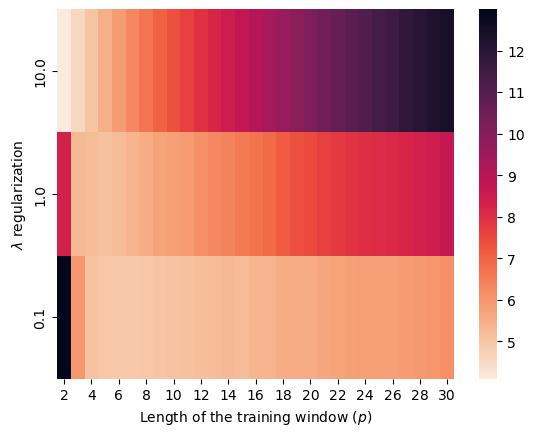
\includegraphics[width=0.9\linewidth]{images/enph_lambda.png}
    \caption{\centering MAPE dependence on the rolling window training length parameter and regularization parameter (Lasso, stock ENPH).}
    \label{fig:1}
\end{figure}
In terms of the parameter $p$, it can be observed that the lowest MAPE values are reported in the
interval of $p \in [4, 8]$. Based on further analyses, we chose $p = 4$ as a constant value. With such 
value of the parameter $p$, the optimal (in terms of all stocks) interval for regularization parameter was identified as $\lambda \in [4, 5]$.
Figure \ref{fig:2} shows an overview of MAPE for the chosen ENPH stock as a function of $\lambda$. 
\begin{figure}[H]
    \centering
    
\includegraphics[width=0.9\linewidth]{images/lambda_lasso.png}
    \caption{\centering MAPE dependence on the rolling window training length parameter (Lasso, stock ENPH).}
    \label{fig:2}
\end{figure}
Such a convex pattern was observed for all analyzed stocks, indicating that the localization of the optimal value of $\lambda$ was
straightforward in all cases.

In the evaluation of the Lasso framework we decided to implement two different approaches. First, we configured the Lasso model with one
universal value of $\overline{\lambda}$ being the arithmetic mean of all optimized values of $\lambda$ of individual stocks. The resulting 
value is $\overline{\lambda} = 4.15$ (referred to as the General model). Second, model with variable value of $\lambda$, is based on identifying
stock and applying its optimized value of $\lambda$ in model (referred to as the Stock-wise model).

The evaluation of these models on the training-validation interval is shown in Table \ref{tab:1}:
\begin{table}[H]
\centering
\resizebox{\columnwidth}{!}{%
\begin{tabular}{|c|c|c|}
\hline
\textbf{Model Type} & \textbf{MAPE (\%)} & \textbf{Dominance (\%)} \\
\hline
General model & 2.297 & 36.16 \\
\hline
Stock-wise model & 2.27 & 35.81 \\
\hline
\end{tabular}
}
\caption{\centering MAPE and dominance values for different settings of the model (Lasso).}
\label{tab:1}
\end{table}
An interesting aspect to note is the ordering of the evaluation metrics for both models. It is possible to
observe higher value of MAPE for the General model; however, this configuration achieves comparatively better dominance. 
Such behaviour may appear counterintuitive, as higher proportion of predictions being closer to the actual 
target values of target variable might yield lower overall deviation.

\subsection{Ridge regression}
Since the model has the same parameters as in the case of Lasso regression, it is possible to employ
the same methodology of hyperparameter tuning.

Figure \ref{fig:3} shows the combined dependence of MAPE on the rolling window parameter $p$ and the regularization parameter $\lambda$ (stock ENPH). Similar to the Lasso, 
this pattern was observed for the vast majority of the analyzed stocks.
\begin{figure}[H]
    \centering
    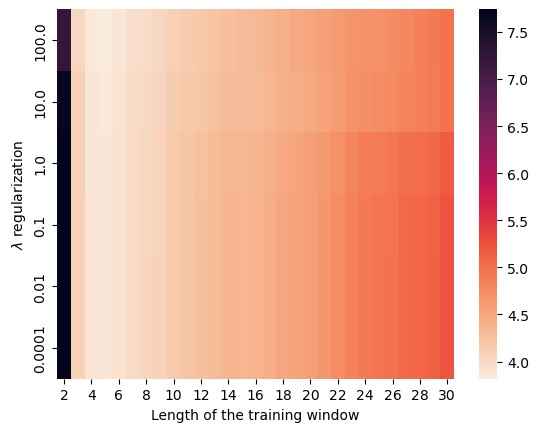
\includegraphics[width=0.9\linewidth]{images/enph_heat_ridge.png}
    \caption{\centering MAPE dependence on the rolling window training length parameter and regularization parameter (Ridge, stock ENPH).}
    \label{fig:3}
\end{figure}
In direct comparison with Figure \ref{fig:1}, likewise a clear segment of near-optimal values can be observed for $p \in [4, 6]$. 
Based on the further experiments with model fitting, we chose the value $p = 4$. 

Furthermore, the dependence of MAPE solely on the $\lambda$ regularization parameter can be analyzed. Figure \ref{fig:4} again shows
a convex pattern for the ENPH stock. 
\begin{figure}[H]
    \centering
    
\includegraphics[width=0.9\linewidth]{images/lambda_ridge.png}
    \caption{\centering MAPE dependence on the rolling window training length parameter (Ridge, stock ENPH).}
    \label{fig:4}
\end{figure}
Even in this case, this pattern was observed in for all analyzed stocks, therefore localizing the optimal value for each stock
was straightforward.

Lastly, for model evaluation, we employed the same approach as in the Lasso framework. The average value of optimal $\lambda$
across all analyzed stocks is $\overline{\lambda} = 211.85$ (referred to as the General model). The approach of using the stock-specific optimal value of $\lambda$
was also preserved (referred to as the Stock-wise model). The evaluation results are presented in Table \ref{tab:2}
\begin{table}[H]
\centering
\resizebox{\columnwidth}{!}{%
\begin{tabular}{|c|c|c|}
\hline
\textbf{Model Type} & \textbf{MAPE (\%)} & \textbf{Dominance (\%)} \\
\hline
General model & 1.791 & 45.08 \\
\hline
Stock-wise model & 1.79 & 45.15 \\
\hline
\end{tabular}
}
\caption{\centering MAPE and dominance values for different settings of the model (Ridge).}
\label{tab:2}
\end{table}
Compared to the results in Table \ref{tab:1}, the ordering of the models is preserved -- the Stock-wise model outperforms the General model
in both metrics. Furthermore, the relative differences between the metric values of the models are smaller compared to 
those in the Lasso framework.

In direct comparison, we observe marginal improvement over the Lasso model. Although the
framework is inferior to the naïve benchmark in terms of dominance, its use demonstrates measurable progress.

\subsection{ARIMA model}
In the case of ARIMA we employed a different approach to hyperparameter tuning compared to the previous two frameworks.
For each rolling window, the initial state $p = 0, d = 0, q = 0$ is set. Incrementally, algorithm
explores the universe of possible settings by exploring the \textit{neighboring} states in the grid. All possible combinations
of integer settings are fitted on the given training data and Bayesian information criterion (BIC) is evaluated \cite{pmdarima}.

Subsequently, the optimal setting based on BIC is chosen. This method is somewhat naïve optimizer and, in terms of time complexity, 
computationally cumbersome. However, for the purposes of this research, this approach is suitable. 

In this case, there is no need to present any dependence of MAPE or dominance
on the chosen model parameters. For each rolling window and for each stock within
it, optimal settings of $p, d, q$ are chosen based on BIC and there is no need to optimize
parameters separately and visualize dependencies similar to the ones in previous
sections.

Finally, in terms of evaluation, such set model achieved average MAPE per stock $\mathbf{1.897 \%}$ and dominance of $\mathbf{58.25 \%}$.
ARIMA was able to overcome all of the analyzed frameworks (even naïve) in terms of model dominance. On the other hand, in terms of MAPE across stocks,
Ridge model achieved better performance. Such result is particularly interesting, as a comparatively
lower MAPE does not necessarily imply higher dominance.

What is more, the dominance result might arise from the fact that in
approximately $66 \%$ of rolling windows across stocks, $p, d, q$ optimization terminated in a
pathological case where $(p,d,q) = (0,1,0)$, which is equivalent to the proposed naïve
benchmark method.

\subsection{Test evaluation}
Last step in the complex predictive analysis is evaluating performance of optimized models on before unseen (test) data sets.
Evaluation results for all the considered model variants is in Table \ref{tab:3}
\begin{table}[H]
\centering
\resizebox{\columnwidth}{!}{%
\begin{tabular}{|c|c|c|}
\hline
\textbf{Model Type} & \textbf{MAPE (\%)} & \textbf{Dominance (\%)} \\
\hline
ARIMA & 1.923 & 56.68 \\
\hline
Ridge (Stock-wise model) & 1.794 & 45.94 \\
\hline
Ridge (General model) & 1.798 & 45.88 \\
\hline
Lasso (General model) & 2.24 & 38.83 \\
\hline
Lasso (Stock-wise model) & 2.31 & 37.1 \\
\hline
\end{tabular}%
}
\caption{Evaluation of tuned models on test interval.}
\label{tab:3}
\end{table}

Performance of models tend to reach similar values as on the training-validation interval -- possibly no overfitting.
Similar values of metrics indicate that models perform relatively stable on both (differently wide) interval of data.

\section{Portfolio management}
With the obtained models, which are capable of producing reliable predictions for the analyzed universe of stocks, the next step
is to employ these models in portfolio optimization. In this paper, a portfolio is defined as a decision-making yielding 
allocation of capital across particular stocks in order to achieve various objectives (e.g., maximum return, minimal risk, etc.).

\subsection{Theoretical foundations}
Allocating capital across a set of stocks to balance the trade-off of asset
volatility and portfolio return can be formulated as an optimization problem. There
are several approaches to properly constructing a portfolio strategy, each requiring
different types of information from the data \cite{portfolio}.

Taking into account having prediction of returns for the next day as a suitable baseline
\textbf{Markowitz mean-variance portfolio} (MVP) was chosen. However, its elementary form 
tends to be impractical in practice \cite{portfolio}.

Its augmented form, introducing transactions costs was adopted. The complete definition of
the used framework is as follows:
\begin{equation*}
\begin{aligned}
\max_{\mathbf{w}_t} \quad 
& \mathbf{w}_t^{\top}\bm{\mu}_t 
- \lambda_{\text{R}} \mathbf{w}_t^{\top}\bm{\Sigma}\mathbf{w}_t 
- \lambda_{T} \|\mathbf{w}_t - \mathbf{w}_{t-1}\|_1 \\
\\
\text{Subject to:} \quad 
& \mathbf{w}_t \geq \mathbf{0}_a \>\>\> \text{and} \>\>\> \mathbf{1}_a^{\top}\mathbf{w}=1,
\end{aligned}
\end{equation*}
where variable $\mathbf{w}_t, \mathbf{w}_{t-1} \in \mathbb{R}^a$, where $a$ is the total number of assets, are vectors
of weights of particular stock assets in portfolio on days $t$ and $t-1$ respectively. Further, $\bm{\Sigma} \in \mathbb{R}^{a \times a}$ is a covariance
matrix of assets, $\lambda_R$ is the risk-aversion hyperparameter and $\lambda_T$ is the unit transaction cost parameter. 
Lastly, for $\mathbf{x} \in \mathbb{R}^t$, $\|\mathbf{x}\|_1 = \sum_{i=1}^{t} \|\mathbf{x}_i\|$ is the L1 or Manhattan norm.

Such extended MVP framework not only balances return and variance of the possible portfolio, but penalizes high volume of transactions, which
in practice imply lower losses \cite{portfolio}.

This allocation framework is used for daily re-allocations, which means that in every trading day optimization is run and weights of single stock assets
vary on daily basis. In all subsequent analyses, configuration with $\lambda_T = 0.01$ is used.
\newline
\par
Subsequently, it is necessary to define crucial evaluation metrics. Using them, comparison of portfolios between each other would be possible and interpretable.

Suppose portfolio is applied on time interval $[1, N]$ and value of the portfolio is a time series $V = V_1, V_2, \ldots, V_N$ 

\textbf{Cumulative annual growth rate}, representing the average percentage return per year, is given as follows \cite{portfolio}:
\begin{equation}
    \label{eq:1}
    \text{CAGR}(V)=\left(\frac{V_N}{V_1}\right)^{\frac{1}{r}} - 1,
\end{equation}
where $r$ denotes number of trading years between $1$ and $N$ timepoints.

Further, to quantify risk and volatility of the portfolio \textbf{annualized volatility} (AV) can be adopted \cite{portfolio}. Let $r_t = \frac{V_t}{V_{t-1}} - 1$ denote return 
on day $t$. Volatility across the given time interval is given as sample standard deviation of $r_1, r_2, \ldots, r_N$ (denoted as $\sigma$). Subsequently, annualized volatility is given as follows:
\begin{equation}
    \label{eq:2}
    \text{AV}(V) = \sigma\sqrt{P},
\end{equation}
where $P$ is the number of trading days per year.

Lastly, one compound metric, based on Equations \eqref{eq:1} and \eqref{eq:2} can be derived \cite{portfolio}. \textbf{Sharpe ratio} stands for return strategy earns per unit risk and is given as:
\begin{equation}
    \text{Sharpe ratio}(V) = \frac{CAGR(V)}{AV(V)}
\end{equation} 

\subsection{Optimization on training-validation interval}
With obtained predictions, the only parameter of the optimization model to tune is $\lambda_R$, steering the risk-aversion.

In Figure \ref{fig:5}, dependence of CAGR on $\lambda_R$ (in Lasso General model) is depicted.
It is possible to observe, that larger $\lambda_R$ (more conservative portfolio) yields larger CAGR.
\begin{figure}[H]
    \centering
    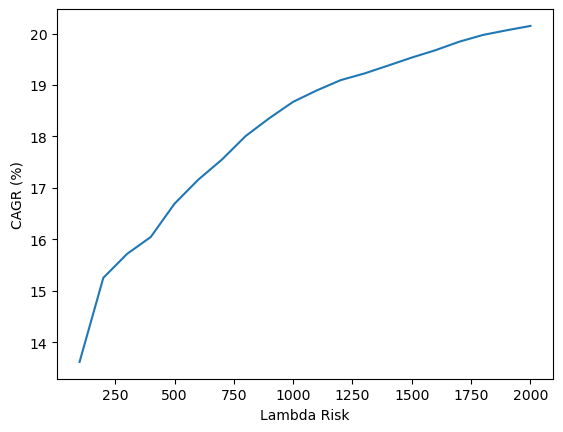
\includegraphics[width=0.9\linewidth]{images/lambda_risk.png}
    \caption{\centering Dependence of portfolio CAGR on risk-aversion parameter (Lasso General model).}
    \label{fig:5}
\end{figure}
On top of that, in terms of CAGR dependence, such course was observed in all three analyzed model frameworks. Each portfolio, backed with predictions made by the particular model, has
growing returns with growing value of $\lambda_R$.

Speaking of AV, unified course is observed as well. Figure \ref{fig:6} shows dependence of AV on the value of $\lambda_R$.
\begin{figure}[H]
    \centering
    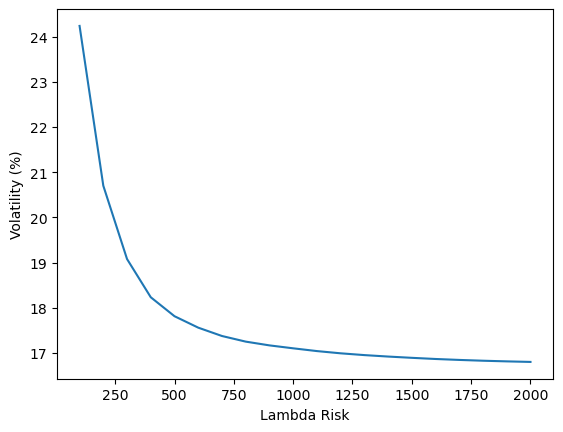
\includegraphics[width=0.9\linewidth]{images/lambda_vol.png}
    \caption{\centering Dependence of portfolio AV on risk-aversion parameter (Lasso General model).}
    \label{fig:6}
\end{figure}
Even in this case, such declining course is observed in all three model frameworks.

Even though pattern is universal for all the frameworks, each implementation was configured differently, as the optimal value was analyzed independently.

In all the models, $\lambda_R$ was chosen as the highest value, beyond which further growth of CAGR or decline of AV has negligible effects.
In cases of Lasso and Ridge, General model variant was evaluated. Overview of configurations is in Table \ref{tab:11}.

\begin{table}[H]
\centering
\begin{tabular}{|c|c|}
\hline
\textbf{Model} & \bm{$\lambda_R$}  \\
\hline
ARIMA & 1000 \\
\hline 
Ridge (SM,GM) & 1200 \\
\hline
Lasso (SM,GM) & 2000 \\
\hline
\end{tabular}
\caption{\centering Portfolio model configuration overview (SM -- Stock-wise model; GM -- General model).}
\label{tab:11}
\end{table}

Evaluation of results on the training-validation interval are overviewed in Table \ref{tab:4}. Naïve strategy stands for portfolio optimization employed 
with naïve benchmark prediction model.
\begin{table}[H]
\centering
\resizebox{\columnwidth}{!}{%
\begin{tabular}{|c|c|c|c|}
\hline
\textbf{Model} & \textbf{CAGR (\%)} & \textbf{AV (\%)} & \textbf{Sharpe ratio} \\
\hline
Naïve & 22.38 & 17.01 & 1.32 \\
\hline
ARIMA & 22.25 & 16.94 & 1.31 \\
\hline
Ridge (SM) & 21.68 & 16.89 & 1.28 \\
\hline
Ridge (GM) & 21.67 & 16.96 & 1.25 \\
\hline
Lasso (SM) & 18.58 & 17.08 & 1.09 \\
\hline
Lasso (GM) & 18.67 & 17.1 & 1.09 \\
\hline
\end{tabular}
}
\caption{\centering Evaluation of tuned models on training-validation interval (SM -- Stock-wise model; GM -- General model).}
\label{tab:4}
\end{table}
As a benchmark was used scenario of investing capital into two indices S\&P 500 and NASDAQ. Performance of these scenarios is 
overviewed in Table \ref{tab:5}.
\begin{table}[H]
\centering
\resizebox{\columnwidth}{!}{%
\begin{tabular}{|c|c|c|c|}
\hline
\textbf{Index name} & \textbf{CAGR (\%)} & \textbf{AV (\%)} & \textbf{Sharpe ratio} \\
\hline
S\&P 500 & 7.69 & 21.75 & 0.35 \\
\hline
NASDAQ & 9.19 & 25.52 & 0.36 \\
\hline
\end{tabular}
}
\caption{\centering Evaluation of benchmark models on training-validation interval.}
\label{tab:5}
\end{table}
Directly comparing results obtained by indices and models, portfolios backed by predictions perfomed marginally better in all reported metrics.
On one hand, during the analyzed period, segment of IT experienced vast rise and this result is expected, but 
on the other hand, NASDAQ index consists mainly from the technology and IT companies, so one could expect
similar performance compared to the model backed strategies \cite{nasdaq}. 

This means, that model backed strategies are capable of being both less risky and better in terms of average annual return.

Overview of ARIMA backed strategy and investments in S\&P 500 and NASDAQ are visualized in Figure \ref{fig:7}.
\begin{figure}[H]
    \centering
    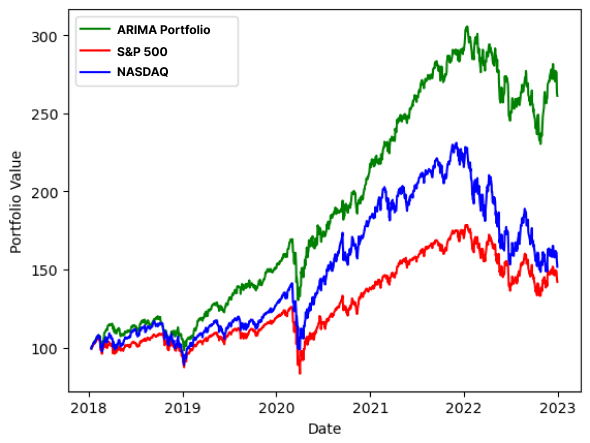
\includegraphics[width=0.9\linewidth]{images/arima_stock.png}
    \caption{\centering Overview of portfolio value across training-validation interval.}
    \label{fig:7}
\end{figure}

\subsection{Test evaluation}
Optimized portfolio strategies were applied on the test interval as well. Throughout results are given in Table \ref{tab:6} together
with performance of benchmark stock indices in the same time period in Table \ref{tab:7}.

% Toto tu treba dokončiť, nech zbehnú testovacie behy SM

\begin{table}[H]
\centering
\resizebox{\columnwidth}{!}{%
\begin{tabular}{|c|c|c|c|}
\hline
\textbf{Model} & \textbf{CAGR (\%)} & \textbf{AV (\%)} & \textbf{Sharpe ratio}\\
\hline
Naïve & 16.48 & 25.20 & 0.65 \\ % DONE
\hline
ARIMA & 15.67 & 25.48 & 0.62 \\ % DONE
\hline
Ridge (SM) & 15.38 & 25.23 & 0.61 \\ % DONE
\hline
Ridge (GM) & 15.29 & 25.24 & 0.6  \\ % DONE
\hline
Lasso (SM) & 16.99 & 25.25 & 0.67 \\ % DONE
\hline
Lasso (GM) & 17.07 & 25.26 & 0.68 \\ % DONE
\hline
\end{tabular}
}
\caption{\centering Evaluation of tuned models on test interval (SM -- Stock-wise model; GM -- General model).}
\label{tab:6}
\end{table}

\begin{table}[H]
\centering
\resizebox{\columnwidth}{!}{%
\begin{tabular}{|c|c|c|c|}
\hline
\textbf{Index name} & \textbf{CAGR (\%)} & \textbf{AV (\%)} & \textbf{Sharpe ratio} \\
\hline
S\&P 500 & 8.35 & 23.1 & 0.36 \\
\hline
NASDAQ & 18.51 & 25.15 & 0.74 \\
\hline
\end{tabular}
}
\caption{\centering Evaluation of benchmark models on test interval.}
\label{tab:7}
\end{table}
Diametrally different evaluations of frameworks is observed. On the shorter test interval,
benchmark indices overcame all the model backed strategies in all metrics. What is more is the opposite
behavior of the models on the interval. While on the training-validation interval, models with the highest dominance
reported the best results; on the test interval quite the opposite was observed.

Paradoxically, the framework with the worst prediction results delivered the best performing portfolio strategy.
This is quite an interesting result in context of the market regime in the time interval. During this period, US market (particularly IT and technology segment)
experienced \textbf{bull market} -- phase in which market in general experiences higher returns and profits \cite{bull}.

This results suggest that MVP backed strategies performed poorly in strong bull market phase. On the other hand, in relatively mediocre phase
between 2017 and 2022 prediction backed strategy performed above expectations. 

On top of that, these results suggest that employing MVP with the proposed naïve prediction benchmark creates resilient portfolio strategy as well. Other model-backed strategies
were unable to outperform the naïve portfolio strategy.

\section{Conclusions}
The results obtained in both prediction modelling and portfolio optimization show that the predictability of the IT segment is relatively low.
This aligns with the Fama \cite{fama1970efficient}, who suggests that stock prices tend to follow random walk development over time.

Even with proper data preparation and feature engineering, most conventional ML frameworks were unable to outperform the
naïve benchmark. However, as mentioned earlier, many studies tend not to compare obtained regression predictions to any benchmark \cite{clanok3, konferencia1}, or compare models only among themselves, stating one as a benchmark \cite{krauss}, which 
may suggest model's false statistical significance.

Interestingly, the study showed counterintuitive fact that in order to build robust and relatively profitable portfolio (compared to conventional indices), being able to
precisely and reliably predict moves on the market is not strictly necessary. The employed MVP framework tends to emphasize the effect of the covariance matrix quadratic form rather than the direct relationship between
weights and expected returns \cite{portfolio}.

Speaking of technical perspective, an essential outcome of the study is the complex and modular data pipeline engine, which is built
on the premises of the introduced methodology. This pipeline is capable of applying all the analyses on any set of financial assets.  

% Keď píšem v pdf-ku
\newpage

\nocite{*}
\bibliographystyle{apalike}
\bibliography{references}

\end{document}
